\chapter[AGES I --- VIR]{AGES I --- \enquote{VIR -- Visual Interactive Reading}}

\section{Introdução}

O projeto "VIR -- Visual
Interactive Reading" busca desenvolver um aplicativo interativo de
leitura para jovens de 12 a 15 anos, alinhado às competências visuais da
geração Alpha. O objetivo é oferecer uma experiência que combina textos
de autores clássicos e contemporâneos com animações, estimulando a
criatividade visual e engajando leitores em formação.

O VIR surge da necessidade identificada em escolas do ensino
fundamental, que enfrentam desafios na formação de leitores engajados.
Baseado em pesquisas acadêmicas e entrevistas com educadores, o
aplicativo contará com funcionalidades como login personalizado, estante
digital, controle de leitura individualizada e recomendação de obras por
faixa etária. Essa abordagem busca complementar a leitura tradicional,
tornando-a mais atrativa e interativa para o público jovem.

\section{Desenvolvimento do Projeto}

\textbf{Stakeholders do Projeto:}

\begin{itemize}
\item
  Hermílio Santos (Professor da Escola de Humanidades - Sociologia -
  PUCRS)
\item
  Paula Vianna (Mestranda em Sociologia - Escola de Humanidades - PUCRS)
\end{itemize}

\textbf{Período de Execução}: Segundo semestre de 2024.

A Figura~\ref{fig:equipe-vir} registra os integrantes que participaram do
projeto VIR.

\begin{figure}[H]
  \centering
  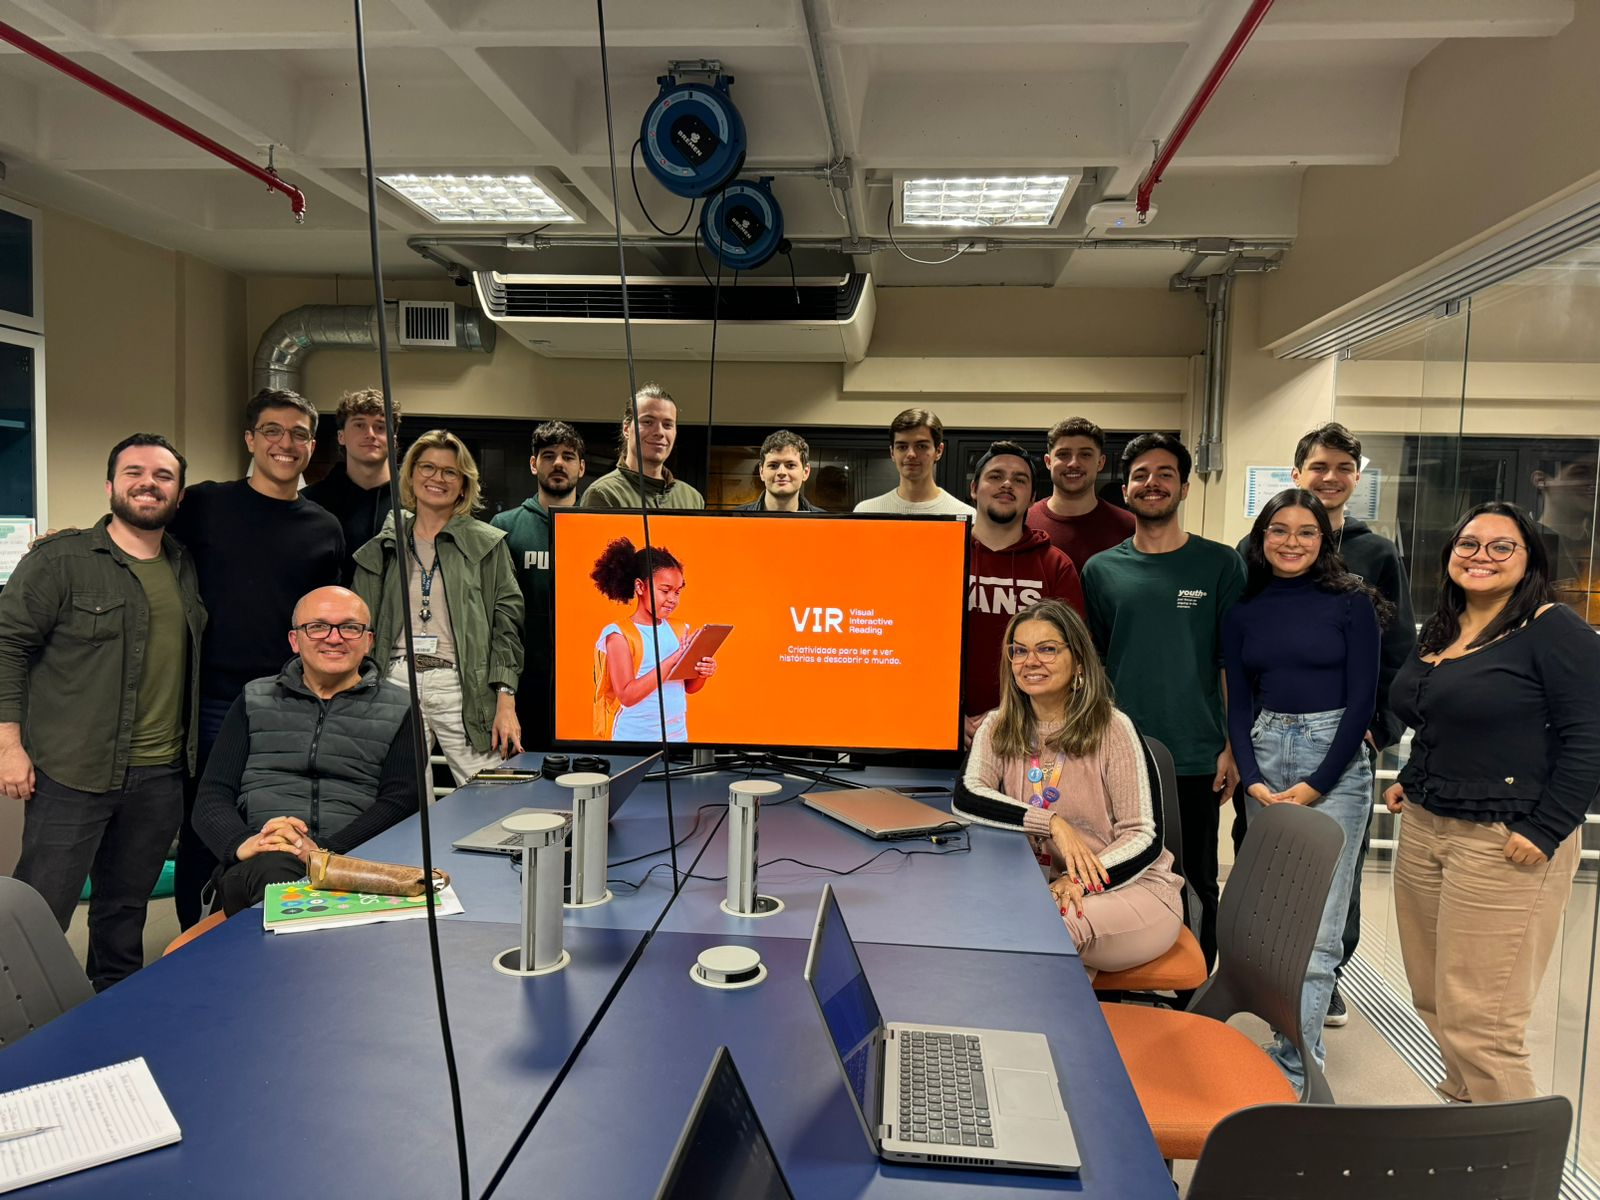
\includegraphics[width=\textwidth]{imagens/VIR/equipe-vir.jpeg}
  \caption{Equipe do projeto VIR}
  \label{fig:equipe-vir}
  \fonte{Acervo pessoal.}
\end{figure}

\begin{enumerate}
\def\labelenumi{\arabic{enumi}.}
\item
  \textbf{Repositório do código Fonte do Projeto}
\end{enumerate}

O código-fonte e a documentação do projeto estão disponíveis na
\href{https://tools.ages.pucrs.br/VIR/vir-wiki/-/tree/main}{wiki do VIR}.

O código fonte está hospedado no GitLab, onde todo o desenvolvimento
colaborativo é gerenciado.

\begin{enumerate}
\def\labelenumi{\arabic{enumi}.}
\setcounter{enumi}{1}
\item
  \textbf{Banco de Dados utilizado}
\end{enumerate}

A documentação do banco de dados está disponível na
\href{https://tools.ages.pucrs.br/VIR/vir-wiki/-/wikis/banco_dados}{wiki do VIR}.

\begin{quote}
Diagrama das tabelas do banco de dados, incluindo usuários, livros,
capítulos, páginas, vídeos e progresso de leitura, ilustrando suas
relações e funcionalidades no projeto VIR.
\end{quote}

\begin{enumerate}
\def\labelenumi{\arabic{enumi}.}
\setcounter{enumi}{2}
\item
  \textbf{Arquitetura utilizada}
\end{enumerate}

Os detalhes arquiteturais estão disponíveis na
\href{https://tools.ages.pucrs.br/VIR/vir-wiki/-/wikis/arquitetura}{wiki do VIR}.

A arquitetura utiliza React no frontend, Flask na \ac{api} e PostgreSQL
como banco de dados \cite{react,postgresql}.
A Figura~\ref{fig:arquitetura-vir} apresenta a organização das camadas e dos
serviços que compunham a arquitetura prevista para o VIR.

\begin{figure}[H]
  \centering
  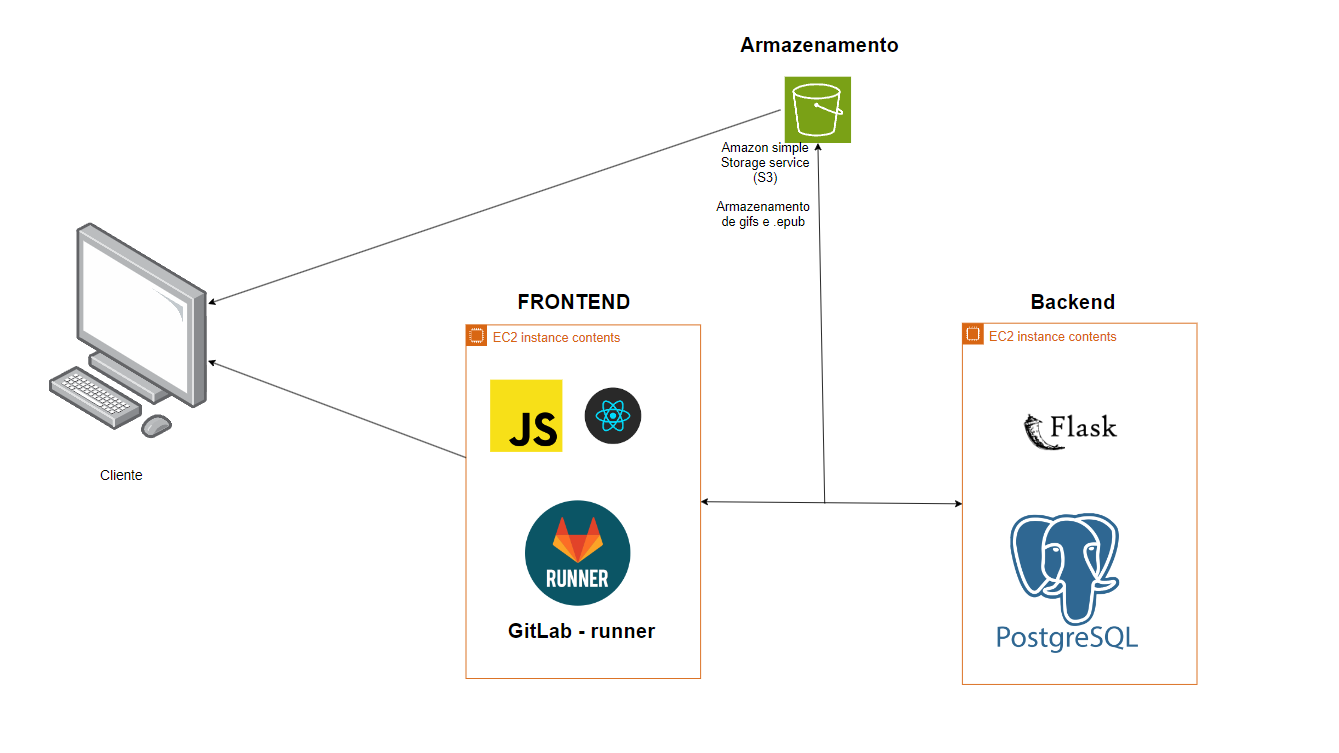
\includegraphics[width=\textwidth]{imagens/VIR/diagrama-arquitetura.png}
  \caption{Arquitetura técnica prevista para o VIR}
  \label{fig:arquitetura-vir}
  \fonte{Acervo do projeto VIR.}
\end{figure}

\begin{enumerate}
\def\labelenumi{\arabic{enumi}.}
\setcounter{enumi}{3}
\item
  \textbf{Protótipos das telas desenvolvidas}
\end{enumerate}

Os protótipos das interfaces estão disponíveis na
\href{https://tools.ages.pucrs.br/VIR/vir-wiki/-/wikis/design_mockups}{wiki do VIR}.

Os mockups do projeto foram feitos no Figma, exibindo o design e fluxo
das interfaces.
A Figura~\ref{fig:arquitetura-informacao-vir} detalha a arquitetura de
informação adotada para os fluxos de leitores, escolas e administradores.

\begin{figure}[H]
  \centering
  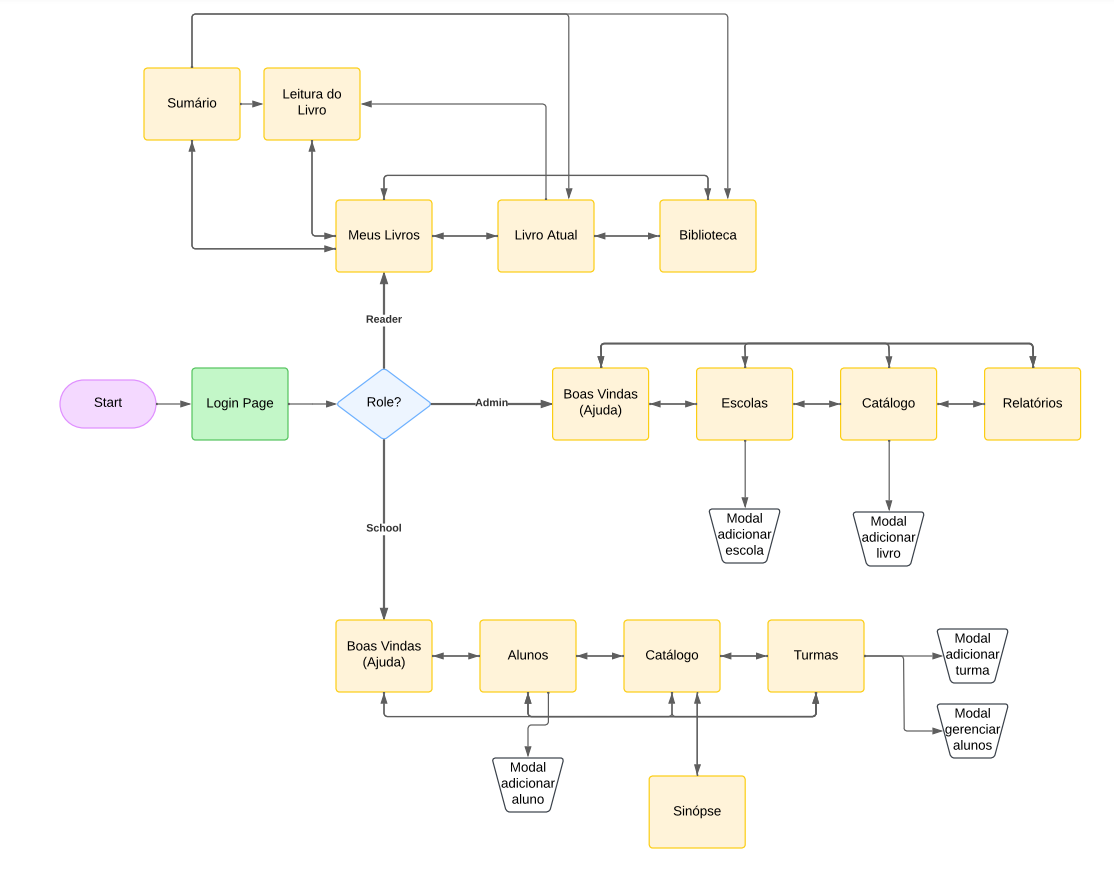
\includegraphics[width=0.9\textwidth]{imagens/VIR/arquitetura-de-informacao.png}
  \caption{Arquitetura de informação do VIR}
  \label{fig:arquitetura-informacao-vir}
  \fonte{Acervo do projeto VIR.}
\end{figure}

\begin{enumerate}
\def\labelenumi{\arabic{enumi}.}
\setcounter{enumi}{4}
\item
  \textbf{Tecnologias Utilizadas}
\end{enumerate}

A configuração detalhada do projeto está disponível na
\href{https://tools.ages.pucrs.br/VIR/vir-wiki/-/wikis/configuracao}{wiki do VIR}.

React (Frontend): Uma biblioteca JavaScript para construir interfaces de
usuário dinâmicas e modernas, permitindo a criação de componentes
reutilizáveis e otimizando a atualização de interfaces por meio do
virtual DOM.

Flask (Backend): Microframework web para Python que permite a criação de
APIs RESTful e aplicações web de forma simples e flexível.

Python: Linguagem de programação usada no backend devido à sua sintaxe
clara e suporte extensivo a bibliotecas.

PostgreSQL: Sistema de gerenciamento de banco de dados relacional,
conhecido por sua robustez e conformidade com padrões SQL.

\section{Atividades desempenhadas pelo aluno no projeto}

\subsection{Sprint 0}

Durante a Sprint 0, meu foco foi compreender os requisitos do cliente e
dar os primeiros passos no desenvolvimento do projeto. As atividades
foram estruturadas para garantir que as bases do projeto estivessem bem
estabelecidas.

\textbf{Atividades Desempenhadas:}

\begin{itemize}
\item
  Preparação para a Reunião Inicial: Desenvolvi perguntas para a reunião
  com o cliente, focando em esclarecer os requisitos, funcionalidades,
  design e aspectos técnicos do sistema.
\item
  Desenvolvimento de Mockups no Figma: Trabalhei na criação de mockups,
  com ênfase no footer do aplicativo. Testei diferentes versões para
  aprimorar a interface e explorei ideias para o scroll da
  funcionalidade de leitura, inspirando-me no estilo de scroll do
  TikTok.
\item
  Configuração do Ambiente de Desenvolvimento: Clonei o repositório do
  GitLab para minha máquina local, ajustei o ambiente, instalei Node.js
  e suas dependências. Fiz a configuração inicial necessária para
  garantir o funcionamento do projeto.
\item
  Revisão de Git e Shell: Para melhorar o fluxo de desenvolvimento,
  revisei o uso do Git e comandos do shell, fundamentais para a
  organização e colaboração no projeto.
\item
  Correção de Vulnerabilidades: Durante a instalação do Node.js,
  encontrei vulnerabilidades que foram corrigidas. Com a ajuda dos
  alunos do AGES IV, entendi que essas vulnerabilidades não impactariam
  o desenvolvimento inicial.
\end{itemize}

\textbf{Ferramentas Utilizadas:}

\begin{itemize}
\item
  Figma: Utilizado para a criação dos mockups e testes de interface.
\item
  GitLab: Ferramenta de versionamento usada para clonar e gerenciar o
  código-fonte do projeto.
\item
  Node.js: Instalado como base para o backend do projeto, com as
  dependências necessárias configuradas.
\item
  Comandos de Git e Shell: Revisados e utilizados para a gestão do
  repositório e ambiente local.
\end{itemize}

\textbf{Contribuições no Desenvolvimento:\\
}\strut \\
Minhas principais contribuições nesta sprint foram a criação dos mockups
iniciais no Figma, com foco em uma interface intuitiva, e a configuração
do ambiente de desenvolvimento. A preparação detalhada para a reunião
inicial com o cliente também ajudou a garantir que as expectativas e
requisitos do sistema fossem claramente definidos.

\subsection{Sprint 1}

Na Sprint 1, o foco foi o desenvolvimento das funcionalidades de
navegação e layout do aplicativo, com destaque para o componente de
footer e o fluxo de leitura, além do estudo contínuo de tecnologias
essenciais para o projeto.

\textbf{Atividades Desempenhadas:}

\begin{itemize}
\item
  Estudo de React: Aprofundei meus conhecimentos em React para
  desenvolver as funcionalidades de navegação do aplicativo. Isso
  incluiu a criação de componentes e o gerenciamento de estado,
  essenciais para o funcionamento do sistema.
\item
  Criação do Footer Component: Desenvolvi o componente de footer na tela
  de estante/biblioteca, garantindo uma navegação eficiente. Fiz ajustes
  no layout utilizando CSS, centralizando e estilizando ícones SVG para
  uma apresentação mais organizada e responsiva.
\item
  Atualização e Configuração do Ambiente: Reconfigurei o ambiente de
  desenvolvimento e criei uma nova branch específica para o
  desenvolvimento do Footer Component. Isso ajudou a manter o controle
  das modificações e facilitou o trabalho colaborativo.
\item
  Implementação Inicial das Rotas: Iniciei a implementação das rotas de
  navegação entre as páginas do aplicativo através dos botões do footer,
  mas não consegui finalizá-las devido à carga de provas e trabalhos
  acadêmicos acumulados.
\item
  Acompanhamento do Time: Embora meu progresso tenha sido limitado,
  acompanhei o desenvolvimento das tarefas da minha squad, garantindo
  que o andamento do projeto continuasse conforme o planejado.
\end{itemize}

\textbf{Ferramentas Utilizadas:}

\begin{itemize}
\item
  React: Utilizado para criar o componente de footer e gerenciar a
  navegação entre as páginas do aplicativo.
\item
  CSS e SVG: CSS foi aplicado para estilizar o layout e centralizar os
  ícones SVG, melhorando o controle visual e responsividade.
\item
  GitLab: Utilizado para gerenciar o repositório do projeto e criar a
  branch dedicada ao Footer Component.
\item
  Node.js: Mantido como base do ambiente de desenvolvimento para
  garantir o funcionamento adequado da aplicação.
\end{itemize}

\textbf{Contribuições no Desenvolvimento:\\
}\strut \\
Minha principal contribuição nesta sprint foi o desenvolvimento do
Footer Component e o início da implementação das rotas de navegação,
essenciais para o fluxo do aplicativo. Apesar das limitações impostas
pela carga acadêmica, garanti que o layout e a estrutura do footer
estivessem finalizados e funcionais, além de contribuir para o andamento
da squad ao acompanhar as tarefas do time.
A Figura~\ref{fig:footer-vir} apresenta as telas de biblioteca e sinopse,
evidenciando a navegação inferior planejada para o aplicativo.

\begin{figure}[H]
  \centering
  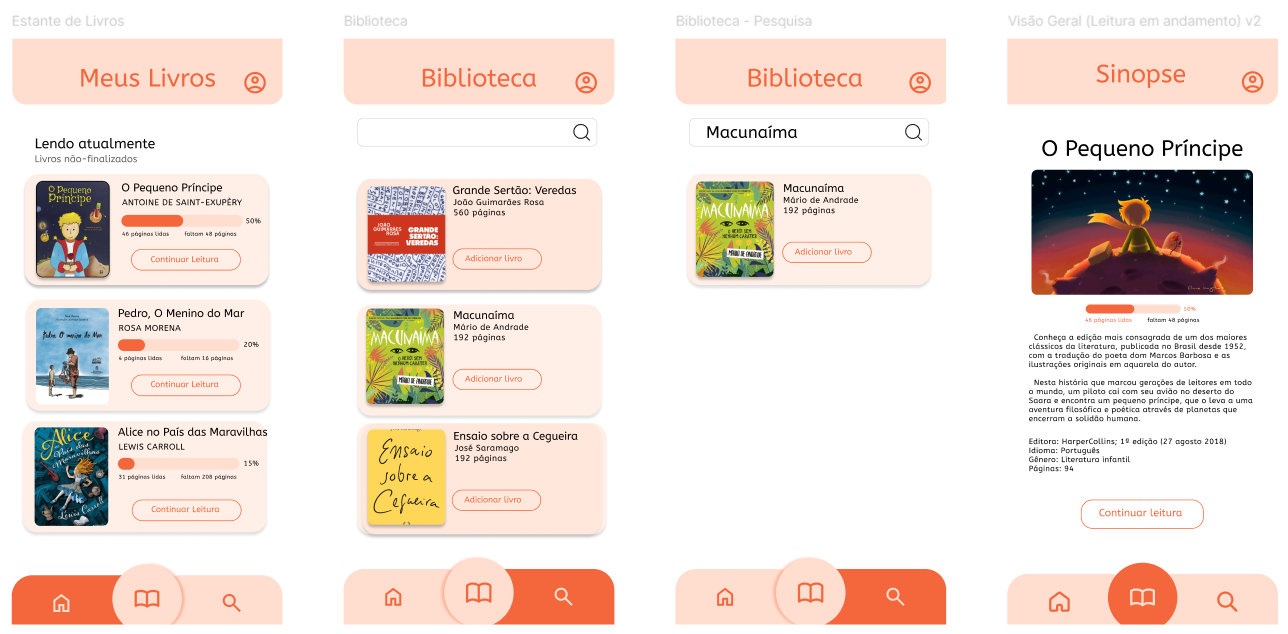
\includegraphics[width=\textwidth]{imagens/VIR/home-footer.png}
  \caption{Telas de biblioteca e navegação inferior do VIR}
  \label{fig:footer-vir}
  \fonte{Acervo do projeto VIR.}
\end{figure}

\subsection{Sprint 2}

Na Sprint 2, o foco foi o desenvolvimento da página de login do VIR,
assegurando funcionalidade, integração com o backend e design intuitivo.
As tarefas incluíram desde a criação e estilização do componente até a
resolução de problemas encontrados durante o desenvolvimento.

\textbf{Atividades Desempenhadas:}

\begin{itemize}
\item
  Criação de uma nova branch: Iniciei o desenvolvimento em uma branch dedicada
  à página de login, derivada da branch \texttt{dev}, garantindo organização e
  controle das modificações.
\item
  Desenvolvimento do Componente Form: Desenvolvi e estilizei o
  componente Form, que incluiu os campos de input para "Email" e
  "Senha", com funcionalidade de censura no campo de senha.
\item
  Criação da Página de Login: Criei e estilizei a página de login,
  integrando o símbolo do VIR e o componente Form, garantindo uma
  interface funcional e intuitiva.
\item
  Configuração e Integração: Implementei o envio de um arquivo JSON
  contendo email e senha ao endpoint correspondente, assegurando
  funcionalidade básica de autenticação.
\item
  Controle de versionamento: Realizei commits das alterações, rebase com a
  branch \texttt{dev} para manter as atualizações e push para o repositório
  remoto.
\item
  Resolução de Problemas no GitLab: Ao fazer um pull request para a
  branch errada (main), corrigi rapidamente com a ajuda dos colegas do
  AGES IV, garantindo a manutenção do fluxo de trabalho
\end{itemize}

\textbf{Ferramentas Utilizadas:}

\begin{itemize}
\item
  GitLab: Utilizado para criação da branch, versionamento do código e
  push das alterações.
\item
  Node.js: Mantido no ambiente de desenvolvimento para suporte ao envio
  do JSON.
\item
  CSS: Usado para estilizar a interface e aprimorar o layout da página
  de login.
\item
  React: Empregado no desenvolvimento do componente Form e na integração
  da página de login.
\end{itemize}

\textbf{Contribuições no Desenvolvimento:}

Minha principal contribuição nesta sprint foi a criação e estilização da
página de login, incluindo o componente Form e a integração com o
backend para envio do JSON. Além disso, a resolução de problemas
relacionados ao GitLab contribuiu para o fluxo de trabalho da equipe,
garantindo organização e eficiência.

\subsection{Sprint 3}

Na Sprint 3, o foco principal foi o desenvolvimento do SchoolFormModal,
com atenção especial à sua estrutura, estilização e funcionalidade, além
de estudos relacionados ao gerenciamento de estado no React.

\textbf{Atividades Desempenhadas:}

\begin{itemize}
\item
  Estruturação do SchoolFormModal: Desenvolvi o modal com header, footer
  e ícone "X" (importado como PNG), além dos botões "Cancelar" e
  "Confirmar".
\item
  Organização de Arquivos CSS: Criei arquivos CSS individuais para cada
  componente do SchoolFormModal, permitindo maior modularidade e
  manutenção.
\item
  Estilização de Botões: Estilizei o botão "Confirmar" com ajustes
  visuais, como cor, sombra e comportamentos específicos para os estados
  hover e click.
\item
  Criação de Componentes Reutilizáveis: Organizei os botões "Cancelar" e
  "Confirmar" como componentes individuais na pasta adminCommons.
\item
  Integração Visual: Adicionei o SchoolFormModal à página da escola
  (escolaPage) para acompanhar o desenvolvimento visual no contexto do
  sistema.
\item
  Estudo de React: Realizei estudos aprofundados sobre o hook useState,
  compreendendo melhor o gerenciamento de estado em componentes
  funcionais.
\item
  Estilização de Inputs: Estilizei os campos de input do modal e revisei
  a estilização geral, adicionando estados hover, focus e pressed aos
  elementos.
\end{itemize}

\textbf{Ferramentas Utilizadas:}

\begin{itemize}
\item
  React: Utilizado para desenvolver o modal, criar componentes
  individuais e implementar o gerenciamento de estado com o hook
  useState.
\item
  CSS: Aplicado na estilização de botões e inputs, com foco em
  modularidade e estados dinâmicos.
\item
  GitLab: Mantido como ferramenta de versionamento para gerenciar as
  alterações no projeto.
\end{itemize}

\textbf{Contribuições no Desenvolvimento:}

Minha principal contribuição nesta sprint foi o desenvolvimento completo
do SchoolFormModal\textbf{,} abrangendo estrutura, estilização e
integração visual na página da escola. Além disso, os estudos sobre o
hook useState aumentaram minha eficiência no gerenciamento de estados em
componentes React.

\subsection{Sprint 4}

Na Sprint 4, o foco foi o desenvolvimento e finalização das
funcionalidades relacionadas à gestão de alunos, incluindo os
componentes Student Modal Form, Student List Component e Student Page,
além de melhorias no controle de estado e correção de problemas
técnicos.

\textbf{Atividades Desempenhadas:}

\begin{itemize}
\item
  Correção do Controle de Estado: Resolvi problemas no controle de
  abertura (isOpen) do modal no componente AlunoPage, ajustando o uso de
  props entre componentes pai e filho.
\item
  Estudo sobre CSS: Realizei estudos sobre propriedades de display, como Grid e
  Flexbox, e sobre estratégias de alinhamento de elementos, aprofundando o
  entendimento sobre as melhores práticas de estilização.
\item
  Desenvolvimento de Componentes: Concluí o desenvolvimento e a
  estilização dos componentes Student Page, Student Modal Form e Student
  List Component, garantindo funcionalidade e integração visual.
\item
  Push e Merge Request: Realizei push e merge request da página de
  aluno, garantindo a sincronização das alterações no repositório
  remoto.
\item
  Investigação de Falhas: Identifiquei e tentei corrigir falhas na
  pipeline devido a branch desatualizada, realizando rebase para
  resolver os conflitos.
\item
  Implementação de Endpoints: Iniciei a implementação dos endpoints da
  página de aluno, enfrentando obstáculos técnicos que ainda precisam de
  resolução.
\end{itemize}

\textbf{Ferramentas Utilizadas:}

\begin{itemize}
\item
  React: Utilizado para corrigir o controle de estado e desenvolver os
  componentes relacionados à página de aluno.
\item
  CSS: Aplicado para estilização dos componentes, com foco no uso
  prático de Grid e Flexbox.
\item
  GitLab: Usado para realizar o push, rebase e merge request das
  alterações no repositório.
\item
  Node.js: Base para a tentativa de implementação dos endpoints.
\end{itemize}

\textbf{Contribuições no Desenvolvimento:}

Minha principal contribuição nesta sprint foi o desenvolvimento e
finalização da Student Page\textbf{,} Student Modal Form e Student List
Component, essenciais para a gestão de alunos. Além disso, resolvi
problemas técnicos relacionados ao controle de estado no modal e
contribuí para a estabilização do fluxo de trabalho no repositório.
A Figura~\ref{fig:gestao-escolas-vir} apresenta a interface de gestão de
escolas, relacionada ao conjunto de funcionalidades administrativas do projeto.

\begin{figure}[H]
  \centering
  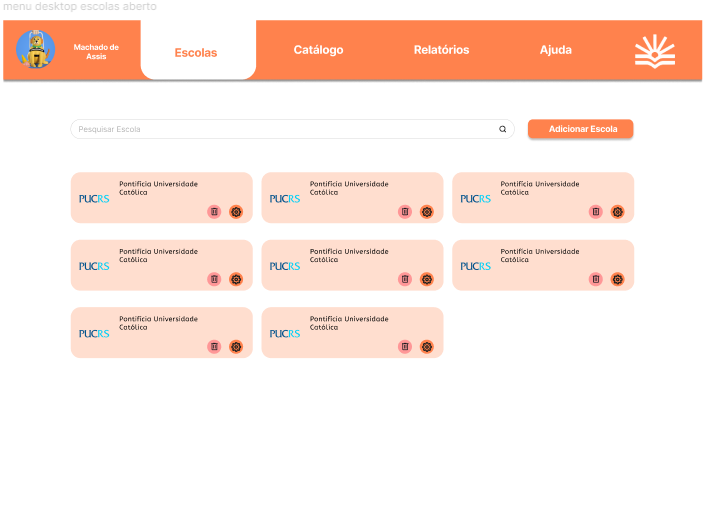
\includegraphics[width=0.85\textwidth]{imagens/VIR/settings-icon.png}
  \caption{Interface de gestão de escolas do VIR}
  \label{fig:gestao-escolas-vir}
  \fonte{Acervo do projeto VIR.}
\end{figure}

\section{Conclusão}

Este projeto se destacou como uma experiência transformadora na minha
trajetória acadêmica, pois me proporcionou uma visão ampla e prática do
fluxo de desenvolvimento de um projeto real. Desde a definição de
requisitos até a entrega de funcionalidades, pude compreender como as
diferentes etapas de um projeto se interconectam, exigindo planejamento,
colaboração e atenção aos detalhes.

O desenvolvimento do VIR exigiu que eu aprofundasse meu entendimento
sobre a estruturação de um projeto como um todo, incluindo a integração
entre o front-end, o back-end e o banco de dados. Trabalhar em um
ambiente dinâmico me permitiu visualizar como essas áreas se comunicam,
como gerenciar estados e como organizar componentes modulares e
reutilizáveis de forma eficiente. Além disso, o uso de ferramentas como
React, GitLab e CSS reforçou a importância de boas práticas de
desenvolvimento e versionamento.

Essa experiência também destacou a relevância de metodologias ágeis para
organizar o trabalho em equipe e garantir entregas contínuas. Aprendi a
lidar com problemas técnicos, como falhas na pipeline e dificuldades de
integração, e a importância de alinhar expectativas com a equipe e
stakeholders. Esse aprendizado me preparou para lidar melhor com a
complexidade de projetos futuros, ampliando minha confiança e
competência técnica.

O desenvolvimento do projeto também me fez perceber a importância de
alinhar a teoria com a prática, exigindo esforço para aplicar
conhecimentos de programação, design e gerenciamento em um contexto
real. No futuro, pretendo aproveitar esse aprendizado para me tornar um
profissional mais completo, capaz de colaborar em projetos que demandem
integração entre diversas áreas e habilidades.


